\title{\bf Gravitational Lensing}

\section{Basics}

Under general relativity, in the presence of mass light is bent by the
curvature of spacetime. On astronomical scales this can cause the
phenomenon of {\it gravitational lensing}. 

\subsection{Point mass lensing}

Understanding lensing begins with the point mass case. It can be shown
that a photon traveling by a point mass, with an impact parameter $r$,
is in the small deflection limit deflected by an angle:
\begin{equation}
\theta_D = \frac{4GM}{rc^2} 
\end{equation}
This differs by a factor of two from the equivalent Newtonian
calculation. An important feature of lensing is that it is achromatic;
i.e., independent of wavelength.

Figure \ref{fig:symmetric} describes the symmetric point lens case and
defines the distances involved. In an analog to the optical thin lens
approximation, we define the {\it source plane} and the {\it lens
  plane}. In the perfectly aligned case the observer sees the source
as a ring surrounding the lens; perfect alignment means an offset
substantially than the source size.  A characteristic quantity of a
lens is radius of this ring, which is the {\it Einstein angle}:
\begin{equation}
\theta_E =  \sqrt{\frac{4GM}{c^2}} \sqrt{\frac{D_{LS}}{D_L D_S}}
\end{equation}
which can be related to the {\it Einstein radius} in the lens plane
$r_E = D_L \theta_E$.

Figure \ref{fig:offset} describes the offset point lens case. If the
source is a point source, this will result in two magnified (and one
highly demagnified) images for the observer. The condition on the
source angle:
\begin{equation}
\beta < \theta_E
\end{equation}
defines the {\it strong lensing} regime. In this regime, the two
images appear near the Einstein ring location. If the source is
extended instead of point-like, it can appear highly distorted in the
strong lensing case.

The opposite case is known as the {\it weak lensing} regime. 

In either case, the distortion of lensing has an effect on the
apparent brightness of the object. The total magnification can be
defined as the increase in the solid angle of the image. This solid
angle increase occurs even if our instrumentation still cannot detect
the extended nature of the image. Because surface brightness (more
technically specific intensity) is conserved in general relativity
this magnification leads to an increase in total flux density.

For multiply imaged sources, the images formed follow different paths
of different distances. This fact leads to a relative delay between
photons that travel different paths. In addition, a different general
relativistic delay is associated with each path, known as the {\it
Shapiro delay}. Fluctuations in the source will appear to the observer
at different times. A measured delay yields a measurement of physical
distance that can in principle be used to determine the distances of
the source and lens.

\subsection{Lensing from extended mass sheets}

On cosmological scales, weak lensing outside the Einstein radius of
individual groups and clusters occurs, but is not well described by
single point mass lensing. We will instead here describe the lensing
as due to a sheet of mass in the lens plane of varying surface
density. 

Let us consider a point in the source plane that (undeflected) would
be at angle $\vec{\beta}$. Let $\vec{x}$ represent the physical
position in the lens plane that the undeflected ray would have passed
through.  The deflection angle is the sum of the contributions of all
the mass in the lens plans:
\begin{equation}
\vec{\theta_D}\left(\vec{x}\right) = \frac{4G}{c^2
D_L}  \int \dd^2 \vec{x}' \Sigma\left(\vec{x}\right) \frac{\vec{x}
- \vec{x}'}{\left|\vec{x} - \vec{x}'\right|^2}
\end{equation}
We can relate the source plane position $\vec{\beta}$ to the observed
angle $\theta$ with the {\it lens equation}:
\begin{equation}
\vec{\beta} = \vec{\theta}
- \frac{D_{LS}}{D_S} \vec{\theta_D}\left(D_L \vec{\theta}\right)
  = \vec{\theta} - \vec{\alpha}
\end{equation}
We can use the above relations to show:
\begin{equation}
\vec{\alpha}
= \frac{1}{\pi} \int \dd^2\vec{\theta}' \kappa\left(\vec{\theta}'\right)
\frac{\vec{\theta} - \vec{\theta}'}
{\left|\vec{\theta} - \vec{\theta}'\right|^2}.
\end{equation}
where we define:
\begin{equation}
\kappa = \frac{\Sigma}{\Sigma_{\rm cr}},
\end{equation}
and:
\begin{equation}
\Sigma_{\rm cr} = \frac{c^2 D_S}{4\pi G D_{LS} D_L}
\end{equation}
The condition $\kappa>1$ leads to multiply imaged sources.

The form of $\vec{\alpha}$ suggests that it can be written as the
gradient of a potential,
\begin{equation}
\vec{\beta} = \vec{\theta} - \vec{\nabla}\psi,
\end{equation}
where
\begin{equation}
\psi
= \frac{1}{\pi} \int \dd^2\vec{\theta}' \kappa\left(\vec{\theta}'\right)
\ln \left|\vec{\theta} - \vec{\theta}'\right|.
\end{equation}
We can also show:
\begin{equation}
\label{eq:poissonlike}
\nabla^2\psi = 2 \kappa
\end{equation}
We can define the Fermat time delay potential as
\begin{equation}
\tau\left(\vec{\theta}; \vec{\beta}\right) =
\frac{1}{2} \left(\vec{\theta} - \vec{\beta}\right)^2
- \psi\left(\vec{\theta}\right),
\end{equation}
and the lens equation can be rewritten as.
\begin{equation}
\vec{\nabla}\tau = 0.
\end{equation}
This result is an expression of the general relativistic version of
Fermat's principle.

\subsection{Weak lensing}

The lens equation can be locally linearized  around $\vec{\beta_0}$:
\begin{equation}
\vec{\beta} = \vec{\beta}_0
+ \frac{\partial \vec{\beta}}{\partial \vec{\theta}} \cdot \left(\vec{\theta}
- \vec{\theta_D} \right), 
\end{equation}
The vector $\vec{\theta}$ and the Jacobian can be written in index form:
\begin{eqnarray}
\vec{\theta} &=& \theta_i {\hat e}_i = \theta_1 {\hat e}_1
+ \theta_2 {\hat e}_2 \cr
{\bf A}\left(\vec{\theta}\right) &=& 
\frac{\partial \vec{\beta}}{\partial \vec{\theta}} = \left(\delta_{ij}
- \frac{\partial^2 \psi}{\partial\theta_i \partial\theta_j}\right)
{\hat e}_i {\hat e}_j.
\end{eqnarray}

The Jacobian is symmetric, so has only three independent parameters,
and we can define three parameters to characterize it, $\kappa$,
$\gamma_1$, and $\gamma_2$:
\begin{equation}
{\bf A} = \left(\begin{array}{cc}
1-\kappa - \gamma_1 & -\gamma_2 \cr
- \gamma_2 & 1-\kappa + \gamma_1
\end{array}\right).
\end{equation}
We do this because, as we are about to show, $\kappa$ (called the {\it
convergence}) is basically the isotropic component of the distortion,
and $\gamma = \gamma_1 + i\gamma_2 = |\gamma| \exp(2i\phi)$ is a shear
term expressing the nonisotropic component, including the rotation of
the image $\phi$.

If you have a circularly symmetric source on sky, this linear
transformation will convert it into an ellipse. You can determine the
parameters of the ellipse from the eigenspace of the of the distortion
matrix. The two eigenvalues are
\begin{equation}
\lambda_{\pm} = (1-\kappa) \pm |\gamma|
\end{equation}
The eigenvector associated with $\lambda_+$ is rotated from ${\hat
e}_1$ towards ${\hat e}_2$ by the angle $\phi$, which is defined by:
\begin{equation}
\cos 2\phi = \frac{\gamma_1}{|\gamma|}
\end{equation}
Based on the eigenvalues, the magnification is:
\begin{equation}
M = \left(\lambda_+ \lambda_-\right)^{-1} = \left[(1-\kappa)^2 -
|\gamma|^2\right]^{-1} 
\end{equation}

In order for $\kappa$ to express an isotropic distortion, then we must
define:
\begin{eqnarray}
\kappa &=& \frac{1}{2}\left(
\frac{\partial^2\psi}{\partial\theta_1^2} +
\frac{\partial^2\psi}{\partial\theta_2^2}\right) \cr
\gamma_1 &=& \frac{1}{2} \left(
\frac{\partial^2\psi}{\partial\theta_1^2} -
\frac{\partial^2\psi}{\partial\theta_2^2}\right),
\end{eqnarray}
and we can further see:
\begin{eqnarray}
\gamma_2 &=& \frac{\partial^2\psi}{\partial\theta_1 \partial\theta_2}.
\end{eqnarray}
Therefore, we can relate the lensing potential curvature to the shear
and convergence of distortions.

We also see why we defined the convergence with $\kappa$, because it
is related to $\psi$ in the same way as the $\kappa$ in the previous
subsection (Equation \ref{eq:poissonlike}). 

In reality, the lensing is integrated through a series of mass sheets
that comprise the three-dimensional density field. In addition, the
convergence due to the mean density is already accounted for in the
cosmological comoving transerve distance, luminosity distance, and
angular diameter distances. The cosmological comoving transverse
distance is that which is relevant to lensing. A rigorous derivation
is beyond our scope here, but the consequence is that the convergence
in some direction for sources at $D=D_S$ can be written as:
\begin{equation}
\kappa(\vec{\theta}, D_S)
= \frac{3 \Omega_m}{2} \int_0^{D_S} \frac{\dd{D_L}}{a(D_L)}
\frac{D_{LS} D_L}{D_S} \delta(\vec{\theta}, D_L)
\end{equation}
where is it understood that $D_L$, $D_{LS}$, and $z_L$ are the
appropriate quantities for a giving lens distance $D_L$. Two important
aspects of this formula are the dependence on $\Omega_m$ and the
weighting factor $D_{LS} D_L$, which tells us which distances do the
most lensing. For a flat universe, $D_{LS}D_L = (D_S - D_L)D_L$, which
has a maximum at $D_L = D_S/2$, so most of the lensing effect is at
from about half the distance of the source. The convergence is also
dependent on the distance of both the lenses and sources, which
therefore need to be known to interpret lensing data accurately.

Weak lensing can be observed through its effects on the size and
brightness of sources (the magnification) or due to the induced change
in ellipticity. Magnification causes a {\it magnification bias} in
flux-limited samples with steep flux counts, because the magnification
will bring a large number of sources from below the (unlensed) flux
limit.  Magnification can also be detected by correlating the number
of background sources against foreground lens galaxies.

The changes in ellipticity can only be observed statistically, because
galaxies at best have random ellipticities (in fact, it is worse as
their ellipticities tend to be aligned, an effect known as {\it
intrinsic alignment}). If you observe an individual galaxy, its
typical ellipticity is $\sim 0.3$ whereas the lensing induced
ellipticity is $<10^{-3}$. One can average over many galaxies along
some line of site to detect a net ellipticity that can be associated
with lensing, which is the ratio of eigenvalues:
\begin{equation}
\frac{\lambda_+}{\lambda_-} = \frac{1-\kappa +  |\gamma|}{1-\kappa -
|\gamma|}
\end{equation}
Since one cannot nearly as easily determine the magnification and
therefore $\kappa$, the ratio in effect one is measuring the {\it
reduced shear}:
\begin{equation}
g = \frac{\gamma}{1-\kappa},
\end{equation}
for which
\begin{equation}
\frac{\lambda_+}{\lambda_-} = \frac{1 +  |g|}{1- |g|}.
\end{equation}

There are two general ways the shear is used. The first is the {\it
cosmic shear}, which looks at shear-shear correlations. This method
yields a fairly direct constraint on the statistics of the total mass
density fluctuations. The second is {\it galaxy-galaxy lensing}
correlations, which cross-correlates known foreground sources with
background shear patterns. In general galaxy-galaxy lensing is usually
easier, because the cross-correlation increases the signal-to-noise
and because it tends to average over systematics. 

The shear-shear correlation is a bit subtle, because there is a
component of the shear transverse to the separation vector, and
cross-wise from it. The treatment of this is beyond our scope
here. The key points are that the shear is interrelated with the
surface mass density. In particular:
\begin{eqnarray}
\gamma &=& \frac{1}{2}\left(\partial\psi_{,11}
- \partial\psi_{,22}\right) + i \partial\psi_{,12} \cr
&=& \frac{1}{\pi} \int \dd^2\vec{\theta}' \kappa\left(\vec{\theta}'\right)
\left[\frac{1}{2}\left(\partial_1\partial_1 - \partial_2 \partial_2\right)
+ i \partial_1 \partial_2\right]
\ln \left|\vec{\theta} - \vec{\theta}'\right] \cr
&=& \frac{1}{\pi} \int \dd^2\vec{\theta}' \kappa\left(\vec{\theta}'\right)
\left( \frac{\theta_2^2 - \theta_1^2 -
2i \theta_1\theta_2}{\theta^4} \right)
\end{eqnarray}
So the shear is related through an integral with the surface mass
density. This integral may be inverted from shear data to yield the
mass density; it is a bit tricky because the kernel is $1/\theta^2$ so
edge and finite volume effects are important (though remember it is in
two-dimensions so this scaling is not as bad as for three dimensions).
It can be further shown that the correlation function and power
spectrum of the shear field can be directly related to the convergence
field, meaning that the statistics of the shear field can be used
directly (without explicitly building a map of $\kappa$).

Galaxy-galaxy lensing typically is used by measuring the mean
tangential shear $\gamma_t$ around identified foreground sources
(usually galaxies or clusters of galaxies). 

\subsection{Microlensing}

A phenomenon called {\it microlensing} occurs when the lensing mass
and background source have a relative angular motion. The background
source increases as it moves through the Einstein radius of the
lens. This increase has a distinctive, achromatic signature, that can
be seen for individual stars in our Galaxy through monitoring.

A related phenomenon also known as microlensing occurs when viewing a
background source through a galactic system. The stars create a
lensing potential surface with distinct cusps that cause fluctuations
in the flux of the background source.

These phenomena can only occur if the background source is physically
smaller than the Einstein radius. Otherwise even if the center of the
source is aligned with the lens, most of the light is well outside the
Einstein radius in the lens plane and is not deflected. This fact
makes it possible to constrain the relative sizes of the background
source in different wavelengths (e.g. radio vs. optical) through
observations of its lensing.

\section{Important numbers}

\section{Key References}

\begin{itemize}
  \item
    \href{http://adsabs.harvard.edu/abs/2000asqu.book.....C}{
    {\it Binney \& Tremaine}
      \citet{cox00a}}, Chapter 5
\end{itemize}

\section{Order-of-magnitude Exercises}

\begin{enumerate} 
\item Typical Einstein angles for stars, galaxies, clusters.
\item Typical delay time
\item Typical shear values
\item Estimate probability of microlensing in galaxy
\end{enumerate}   

\section{Analytic Exercises}

\begin{enumerate}
\item GR calculation of lensing offset
\item For a symmetric, point mass lens, derive the angular radius of the image
    that is formed, called the Einstein angle.
\begin{answer}
Using the notation in Figure \ref{fig:symmetric}, geometrically it
must be that:
\begin{equation}
\theta_D = \theta_S + \theta_E
\end{equation}
Under the small angle approximation, therefore:
\begin{equation}
\theta_D = r_E \left(\frac{1}{D_L} + \frac{1}{D_{LS}}\right) =
r_E \frac{D_S}{D_{LS} D_L} 
\end{equation}
Therefore:
\begin{equation}
r_E = \frac{D_{LS} D_L}{D_S} \theta_D.
\end{equation}
Again using the small angle approximation, the impact parameter is
$r_E$, so we can write:
\begin{equation}
r_E = \frac{D_{LS} D_L}{D_S} \frac{4GM}{r_Ec^2}
\end{equation}
and solve for:
\begin{equation}
r_E = \sqrt{\frac{4GM}{c^2} \frac{D_{LS} D_L}{D_S}}
\end{equation}
The Einstein angle can then be calculated (again using small angles):
\begin{equation}
\theta_E = \sqrt{\frac{4GM}{c^2} \frac{D_{LS}}{D_S D_L}}
\end{equation}
\end{answer}

\item Calculate the location of the two magnified images that form when the
source is offset from the point lens.
\begin{answer}
Using the notation in Figure \ref{fig:offset}, we have:
\begin{equation}
r_I = r_S + r_D,
\end{equation}
and therefore:
\begin{eqnarray}
\theta_\pm D_S &=& \beta D_S + D_{LS} \theta_D \cr
\theta_\pm &=& \beta + \frac{D_{LS}}{D_S} \frac{4GM}{r_\pm c^2} \cr
&=& \beta + \frac{D_{LS}}{D_S D_L} \frac{4GM}{\theta_\pm c^2} \cr
&=& \beta + \frac{\theta_E^2}{\theta_\pm}
\end{eqnarray}
Then we can rearrange this to:
\begin{equation}
\theta_\pm^2 - \beta \theta_\pm - \theta_E^2 = 0 
\end{equation}
with the solutions:
\begin{equation}
\theta_\pm = \frac{\beta \pm \sqrt{\beta^2 + 4\theta_E^2}}{2}
\end{equation}
For the strong-lensing limit $\beta \ll \theta_E$, this leads to:
\begin{equation}
\theta_\pm = \pm \theta_E + \frac{\beta}{2}
\end{equation}
For the weak-lensing limit $\beta \gg \theta_E$:
\begin{equation}
\theta_\pm
= \beta \left(\frac{1}{2} \pm \frac{1}{2} \sqrt{1+
\frac{4\theta_E^2}{\beta^2}}\right) 
\end{equation}
and we find:
\begin{eqnarray}
\theta_+ &\approx& \beta + \frac{\theta_E^2}{\beta} \cr
\theta_- &\approx& - \frac{\theta_E^2}{\beta}
\end{eqnarray}
\end{answer}
\item In the weak lensing limit for a point mass lens,  what is the
magnification?
\begin{answer}
Consider a source at $\beta$, with a size in the radial and tangential
directions of $\dd\beta$ and $\dd\phi$ (for the polar coordinate
$\phi$). Its unlensed area is:
\begin{equation}
A_S = \beta \dd\beta \dd\phi
\end{equation}
The area of each lensed image is:
\begin{equation}
A_\pm = \left| \theta_\pm\right| \dd\theta_\pm \dd\phi
= \left| \theta_\pm\right| \left|\frac{\dd\theta_\pm}{\dd\beta}\right| \dd\beta\dd\phi
= \left|\frac{\theta_\pm}{\beta}\right| \left|\frac{\dd\theta_\pm}{\dd\beta}\right| A_S
\end{equation}
Then:
\begin{equation}
M = \frac{A_+ + A_-}{A_S} = \frac{1+
2\theta_E^2/\beta^2}{\sqrt{1+4\theta_E^2/\beta^2} }
\end{equation}
\end{answer}
\item Critical surface density case
\item Derive shear and magnification properties
\end{enumerate}

\section{Numerics and Data Exercises}

\begin{enumerate}
\item Modeling of lens system
\item Specific strong lenses
\item Measurements of shear
\end{enumerate}

\bibliographystyle{apj}
\bibliography{exex}  

\begin{figure}
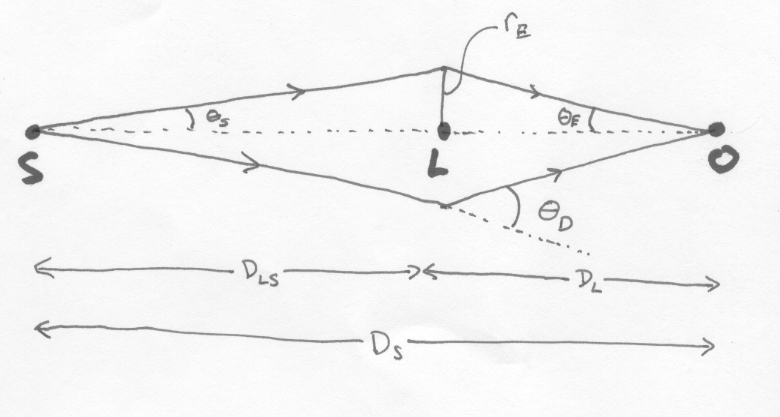
\includegraphics[width=0.9\textwidth]{figures/symmetric_lens.jpg}
\caption{\label{fig:symmetric} Geometry for symmetric point mass lens.}
\end{figure}

\begin{figure}
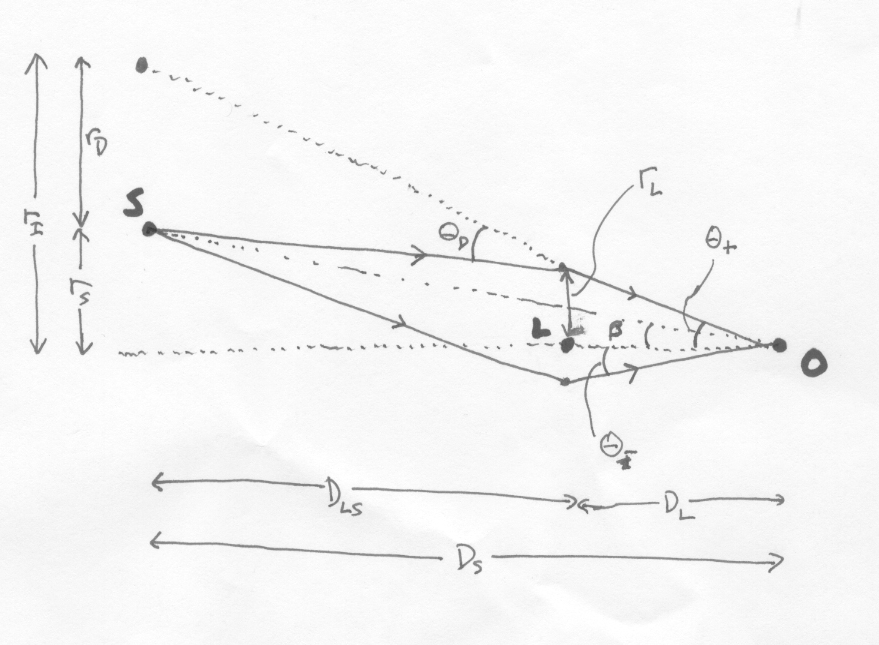
\includegraphics[width=0.9\textwidth]{figures/offset_lens.jpg}
\caption{\label{fig:offset} Geometry for offset point mass lens.}
\end{figure}
